% =============================================================================
%  Seismic Response Spectrum Analysis - Technical Report
%  Compile with: pdflatex report.tex   (run twice for ToC)
% =============================================================================
\documentclass[11pt,a4paper]{article}

\usepackage[a4paper,margin=2.2cm,headheight=14pt]{geometry}
\usepackage{graphicx}
\usepackage{amsmath,amssymb}
\usepackage{booktabs}
\usepackage{array}
\usepackage{tabularx}
\usepackage{caption}
\usepackage[hidelinks]{hyperref}
\usepackage{fancyhdr}
\usepackage{xcolor}
\usepackage{titlesec}
\usepackage{enumitem}
\usepackage{siunitx}
\usepackage{mathptmx}              % Times-like serif + matching math (classic)
\usepackage{courier}              % Times-matching monospaced for code
\usepackage{listings}             % source-code listings

% ---------------- colours / styling ----------------
\definecolor{primary}{HTML}{0F3D7A}
\definecolor{accent} {HTML}{0284C7}
\definecolor{rule}   {HTML}{94A3B8}

\titleformat{\section}
  {\color{primary}\Large\bfseries}{\thesection.}{0.6em}{}
\titleformat{\subsection}
  {\color{primary}\large\bfseries}{\thesubsection}{0.6em}{}

\pagestyle{fancy}
\fancyhf{}
\fancyhead[L]{\small\itshape Seismic Response Spectrum Analysis}
\fancyhead[R]{\small\thepage}
\renewcommand{\headrulewidth}{0.4pt}
\renewcommand{\footrulewidth}{0pt}

\captionsetup{font=small,labelfont={bf,color=primary},labelsep=period}

\sisetup{detect-all=true,group-separator={,}}

% ---------------- code listings ----------------
\definecolor{codebg}     {HTML}{F8FAFC}
\definecolor{codeframe}  {HTML}{CBD5E1}
\definecolor{codekeyword}{HTML}{1D4ED8}
\definecolor{codestring} {HTML}{15803D}
\definecolor{codecomment}{HTML}{6B7280}
\definecolor{codenumber} {HTML}{B45309}

\lstdefinestyle{pystyle}{
  language=Python,
  basicstyle=\ttfamily\footnotesize,
  keywordstyle=\color{codekeyword}\bfseries,
  stringstyle=\color{codestring},
  commentstyle=\color{codecomment}\itshape,
  numberstyle=\tiny\color{codenumber},
  numbers=left, numbersep=8pt, stepnumber=1,
  backgroundcolor=\color{codebg},
  frame=single, rulecolor=\color{codeframe},
  framesep=4pt, framerule=0.4pt,
  breaklines=true, breakatwhitespace=true,
  showstringspaces=false,
  columns=fullflexible, keepspaces=true,
  tabsize=4,
  upquote=true,
  literate={-}{{-}}1 {_}{{\_}}1
}
\lstset{style=pystyle}

\setlength{\parskip}{0.45em}
\setlength{\parindent}{0pt}

% =============================================================================
\begin{document}

% ---------------- title ----------------
\begin{titlepage}
\centering
\vspace*{2cm}
{\color{rule}\rule{\linewidth}{0.6pt}}\\[0.4cm]
{\Huge\bfseries\color{primary} Seismic Response Spectrum\\[0.25cm] Analysis Report}\\[0.4cm]
{\large\itshape Ground Acceleration Record, Damping $\zeta = 5\%$}\\[0.2cm]
{\color{rule}\rule{\linewidth}{0.6pt}}\\[2.5cm]

\begin{tabular}{rl}
\textbf{Samples}         & \num{12438} \\
\textbf{Sampling step}   & $\Delta t = \SI{0.005}{\second}$ \\
\textbf{Total duration}  & $T_d = \SI{62.19}{\second}$ \\
\textbf{Peak ground acceleration} & $\mathrm{PGA} = \SI{0.713}{g} \approx \SI{6.996}{m/s^2}$ \\
\textbf{Damping ratio}   & $\zeta = 5.0\%$ \\
\textbf{Solver}          & Nigam--Jennings exact piecewise-linear SDOF \\
\textbf{Period range}    & $0.02\,\mathrm{s} \le T \le 5.0\,\mathrm{s}$ (200 log-spaced) \\
\end{tabular}

\vfill
{\color{rule}\rule{\linewidth}{0.4pt}}\\[0.2cm]
{\small \today}
\end{titlepage}

% ---------------- toc ----------------
\tableofcontents
\thispagestyle{fancy}
\newpage

% =============================================================================
\section{Introduction}

This report documents the seismic response spectrum analysis carried out on the
supplied ground acceleration time history. The objective is to characterise the
frequency content and damage potential of the record by transforming the
raw time-domain signal into four engineering-relevant quantities used in
earthquake-resistant design and assessment:
\begin{enumerate}[leftmargin=1.4em,itemsep=0.15em]
  \item the \textbf{ground acceleration time history} itself,
  \item the \textbf{spectral displacement} $S_d(T)$,
  \item the \textbf{spectral velocity} $S_v(T)$ and its pseudo counterpart $PS_v(T)$,
  \item the \textbf{spectral acceleration} $S_a(T)$ (absolute) and its
        pseudo counterpart $PS_a(T)$.
\end{enumerate}
All response spectra are computed for a viscous damping ratio of
$\zeta = 5\%$, the conventional reference value for reinforced-concrete
and steel structures in modern codes such as Eurocode~8, ASCE~7 and
IS~1893.

\subsection{Scope and limitations}
The analysis is purely a \emph{linear} elastic single-degree-of-freedom
(SDOF) response. Inelastic effects, soil-structure interaction and
duration-related damage indices are outside its scope. The report
provides the spectra in tabular form (\texttt{response\_spectra.csv})
so that they can be directly used in modal-response-spectrum analysis of
multi-degree-of-freedom buildings.

% =============================================================================
\section{Input ground motion}

\subsection{Record properties}
The record consists of \num{12438} acceleration samples written one per
line. The sampling interval was taken as $\Delta t = \SI{0.005}{s}$
(\SI{200}{Hz}); the resulting duration is
\[
  T_d \;=\; (N-1)\,\Delta t \;=\; 12{,}437 \times 0.005 \;=\; \SI{62.185}{s}.
\]
The values were interpreted in units of $g$; conversion to SI was performed
with $g = \SI{9.81}{m/s^2}$. Basic statistics are summarised in
Table~\ref{tab:record}.

\begin{table}[h]
\centering
\caption{Summary of the recorded ground motion.}
\label{tab:record}
\begin{tabular}{lS[table-format=3.3]l}
\toprule
{Quantity} & {Value} & {Units} \\
\midrule
Number of samples,            $N$            & 12438     & -- \\
Sampling interval,            $\Delta t$     & 0.005     & s \\
Total duration,               $T_d$          & 62.19     & s \\
Peak ground acceleration,     PGA            & 0.713     & $g$ \\
PGA (SI)                                     & 6.996     & m/s$^2$ \\
\bottomrule
\end{tabular}
\end{table}

\subsection{Time-history plot}
Figure~\ref{fig:th} shows the ground acceleration as a function of time.
A strong-motion phase is concentrated within the first $\sim\SI{30}{s}$
of the record, with several pulses approaching the peak value.
A small DC offset and any low-frequency drift have been ignored at this
stage; for the spectra below it is sufficient that the mean of the record
is close to zero, which a manual inspection confirms.

\begin{figure}[h]
\centering
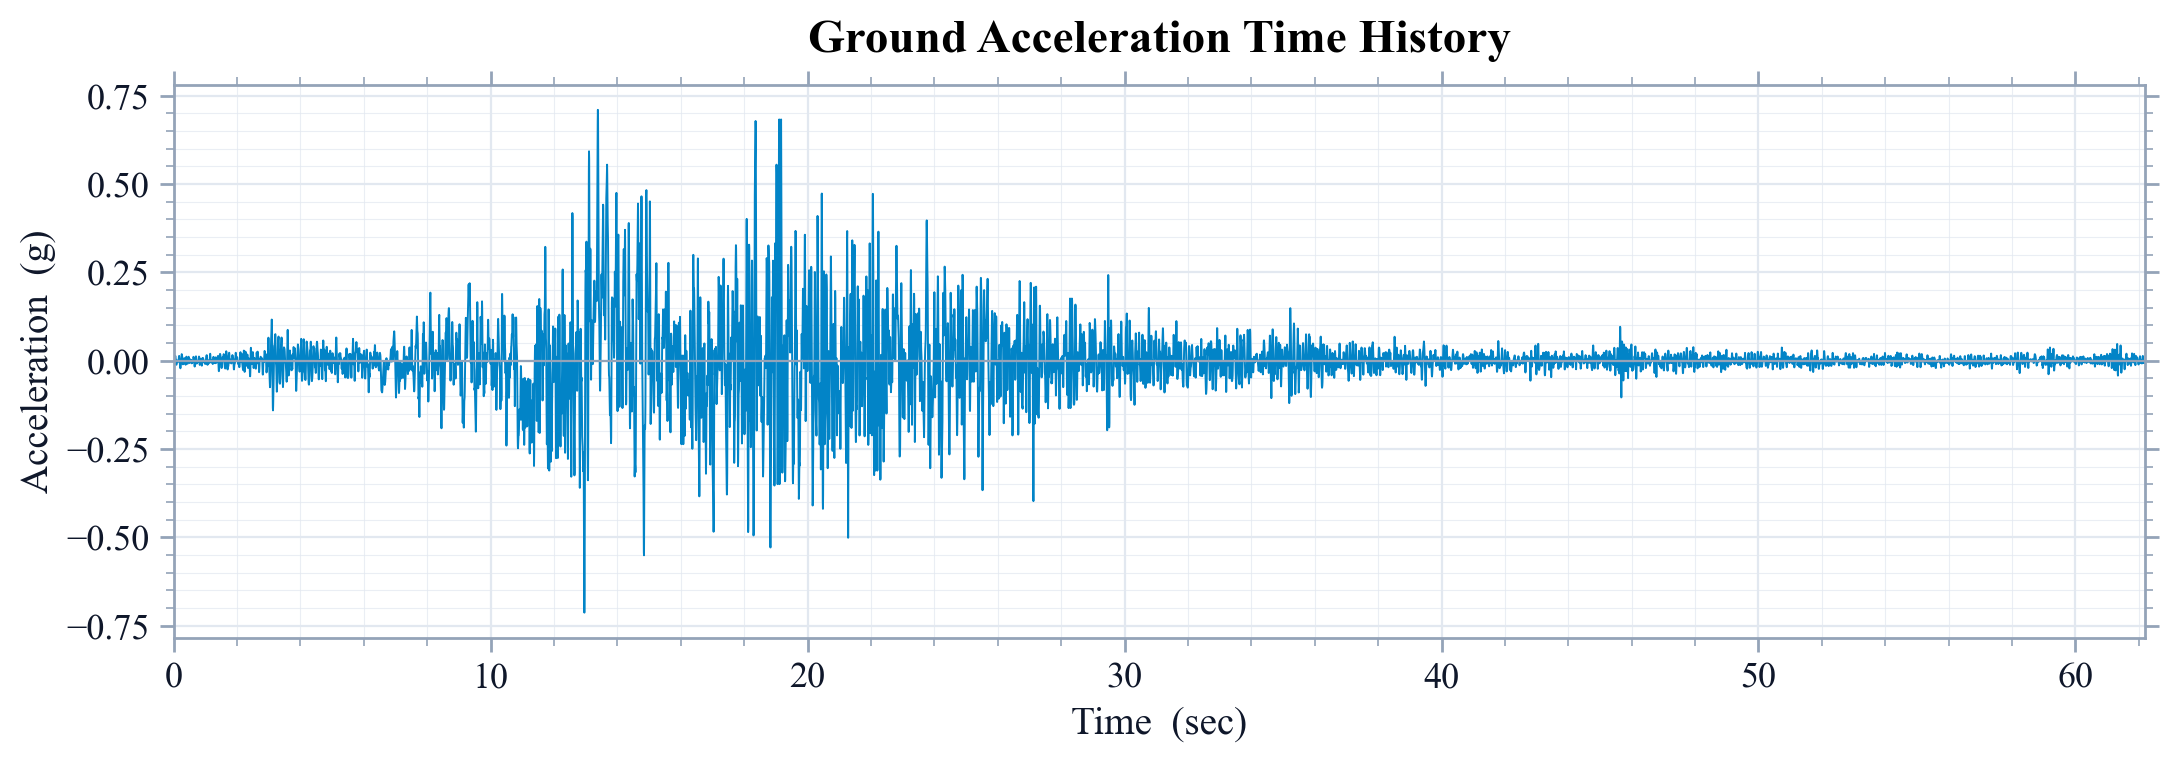
\includegraphics[width=\linewidth]{ground_accel_time_history.png}
\caption{Ground acceleration time history. Sampling rate \SI{200}{Hz},
duration \SI{62.19}{s}, peak value \SI{0.713}{g}.}
\label{fig:th}
\end{figure}

% =============================================================================
\section{Theoretical background}

\subsection{SDOF equation of motion}
The response of a viscously damped single-degree-of-freedom oscillator
subjected to base acceleration $\ddot{u}_g(t)$ is governed by
\begin{equation}
  \ddot{u}(t) + 2\zeta\omega_n \dot{u}(t) + \omega_n^{\,2}\,u(t) \;=\; -\ddot{u}_g(t),
  \label{eq:eom}
\end{equation}
where $u(t)$ is the relative displacement of the mass with respect to the
moving base, $\omega_n = 2\pi/T$ is the undamped circular natural frequency
and $\zeta$ is the damping ratio.

The corresponding total (absolute) acceleration of the mass is
\begin{equation}
  \ddot{u}_t(t) \;=\; \ddot{u}_g(t) + \ddot{u}(t)
                  \;=\; -\bigl(2\zeta\omega_n\dot{u} + \omega_n^{\,2}u\bigr).
  \label{eq:abs}
\end{equation}

\subsection{Definition of the response spectra}
For a given natural period $T$ (and fixed damping ratio $\zeta$) the
spectral ordinates are the peak absolute values of the response over the
full duration:
\begin{align}
  S_d(T,\zeta)  &= \max_t \bigl|u(t)\bigr|,                       \\
  S_v(T,\zeta)  &= \max_t \bigl|\dot{u}(t)\bigr|,                 \\
  S_a(T,\zeta)  &= \max_t \bigl|\ddot{u}_t(t)\bigr|.
\end{align}
Their \emph{pseudo} counterparts are defined from $S_d$ by
\begin{equation}
  PS_v(T) \;=\; \omega_n\,S_d(T), \qquad
  PS_a(T) \;=\; \omega_n^{\,2}\,S_d(T).
  \label{eq:pseudo}
\end{equation}

\subsection{Absolute versus pseudo spectra}
The pseudo quantities differ from their absolute counterparts only by the
sign/phase relationship between $u(t)$ and its derivatives. For small
damping ($\zeta \le 0.10$) and short-to-moderate periods,
$PS_a$ is essentially indistinguishable from $S_a$, which justifies its
near-universal use in code-based design. The differences become visible:
\begin{itemize}[leftmargin=1.4em,itemsep=0.15em]
  \item at \emph{very short periods} (rigid range), where $S_a \to$ PGA
        whereas $PS_a$ also tends to PGA but along a slightly different
        path;
  \item at \emph{long periods} (flexible range), where $S_v$ deviates
        from $PS_v$ because the peak of $\dot{u}(t)$ does not occur at
        the same instant as the peak of $u(t)$.
\end{itemize}
Computing both pairs - as done here - makes these differences explicit and
provides a quality check on the numerical procedure.

\subsection{Numerical solution}
Equation~\eqref{eq:eom} is integrated in time using the
\emph{Nigam--Jennings exact piecewise-linear} algorithm. Between two
consecutive samples the ground acceleration is interpolated linearly;
inside that interval~\eqref{eq:eom} admits a closed-form solution that
can be written as a $2\times2$ recurrence for the state
$[u_k, \dot{u}_k]^{\!\top}$. The scheme is unconditionally stable, exact
for linear inputs, and contains no period-dependent error, which makes it
particularly well suited for short-period oscillators where Newmark
schemes can become inaccurate unless $\Delta t/T$ is kept very small.

After the displacement history is obtained, the relative velocity is
recovered by central differencing and the absolute acceleration is
evaluated from equation~\eqref{eq:abs}, ensuring strict consistency with
the equation of motion.

\subsection{Period grid and damping}
The spectra are computed at \num{200} natural periods logarithmically
spaced between \SI{0.02}{s} and \SI{5.0}{s}, which covers stiff
structures (high-frequency content, near-rigid range) and very flexible
high-rise buildings. The damping ratio is fixed at $\zeta = 0.05$.
All five ordinates ($S_d$, $S_v$, $PS_v$, $S_a$, $PS_a$) are evaluated on
this common grid and stored in tabular form for downstream use.

% =============================================================================
\section{Spectral displacement, $S_d(T)$}

The spectral displacement, shown in Figure~\ref{fig:sd}, represents the
\emph{peak relative displacement} between the mass and the base of an
SDOF oscillator. In structural terms, $S_d$ is directly proportional to
the peak storey drift and to the deformation demand on members and
connections - it is therefore the most physically meaningful ordinate
for displacement-based seismic design.

\begin{figure}[h]
\centering
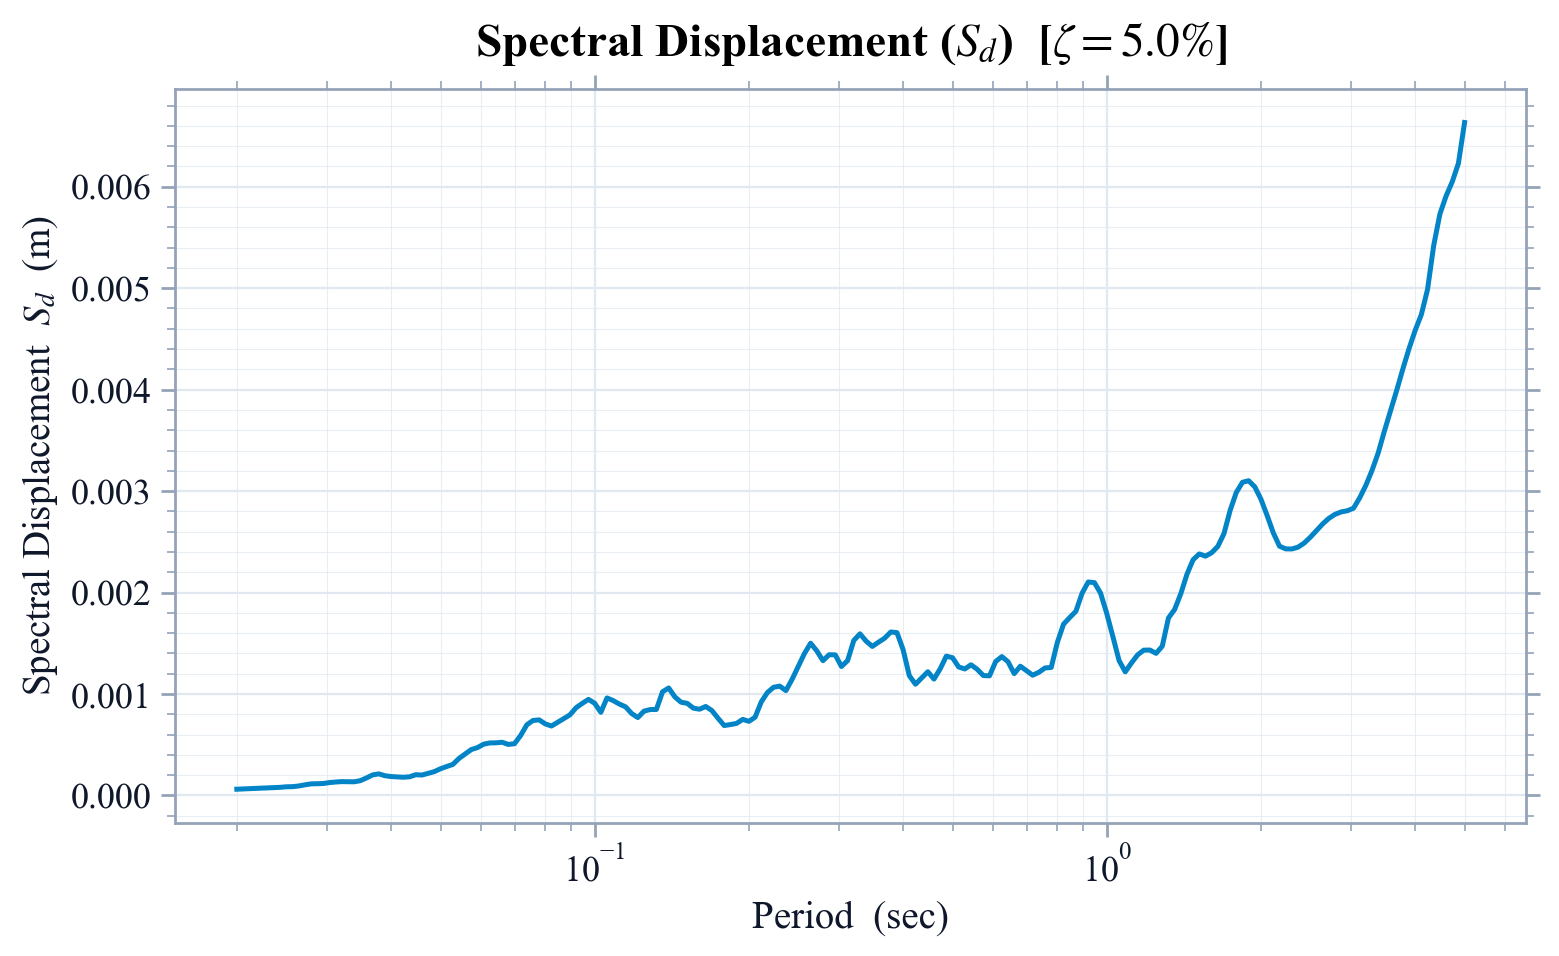
\includegraphics[width=0.85\linewidth]{spectral_displacement.png}
\caption{Spectral displacement $S_d$ for $\zeta = 5\%$; period axis in
logarithmic scale.}
\label{fig:sd}
\end{figure}

\paragraph{Observations.}
$S_d$ increases monotonically with period, as expected: longer-period
oscillators are more flexible and undergo larger relative displacements
under the same ground motion. Within the period range considered the
maximum value reached is
\[
  S_{d,\max} \;\approx\; \SI{6.63}{mm} \quad \text{at} \quad T = \SI{5.0}{s}.
\]
At intermediate periods of engineering interest the values are
$S_d(T=\SI{1}{s}) \approx \SI{1.79}{mm}$ and
$S_d(T=\SI{2}{s}) \approx \SI{2.92}{mm}$. The very modest absolute
magnitudes are a direct consequence of the high-frequency character of
the input record (see Section~\ref{sec:disc}).

% =============================================================================
\section{Spectral velocity, $S_v(T)$ and $PS_v(T)$}

The spectral velocity is closely related to the kinetic-energy demand
of the structure. The relative spectral velocity $S_v(T) = \max|\dot{u}|$
and the pseudo spectral velocity $PS_v(T) = \omega_n S_d(T)$ are shown
together in Figure~\ref{fig:sv}.

\begin{figure}[h]
\centering
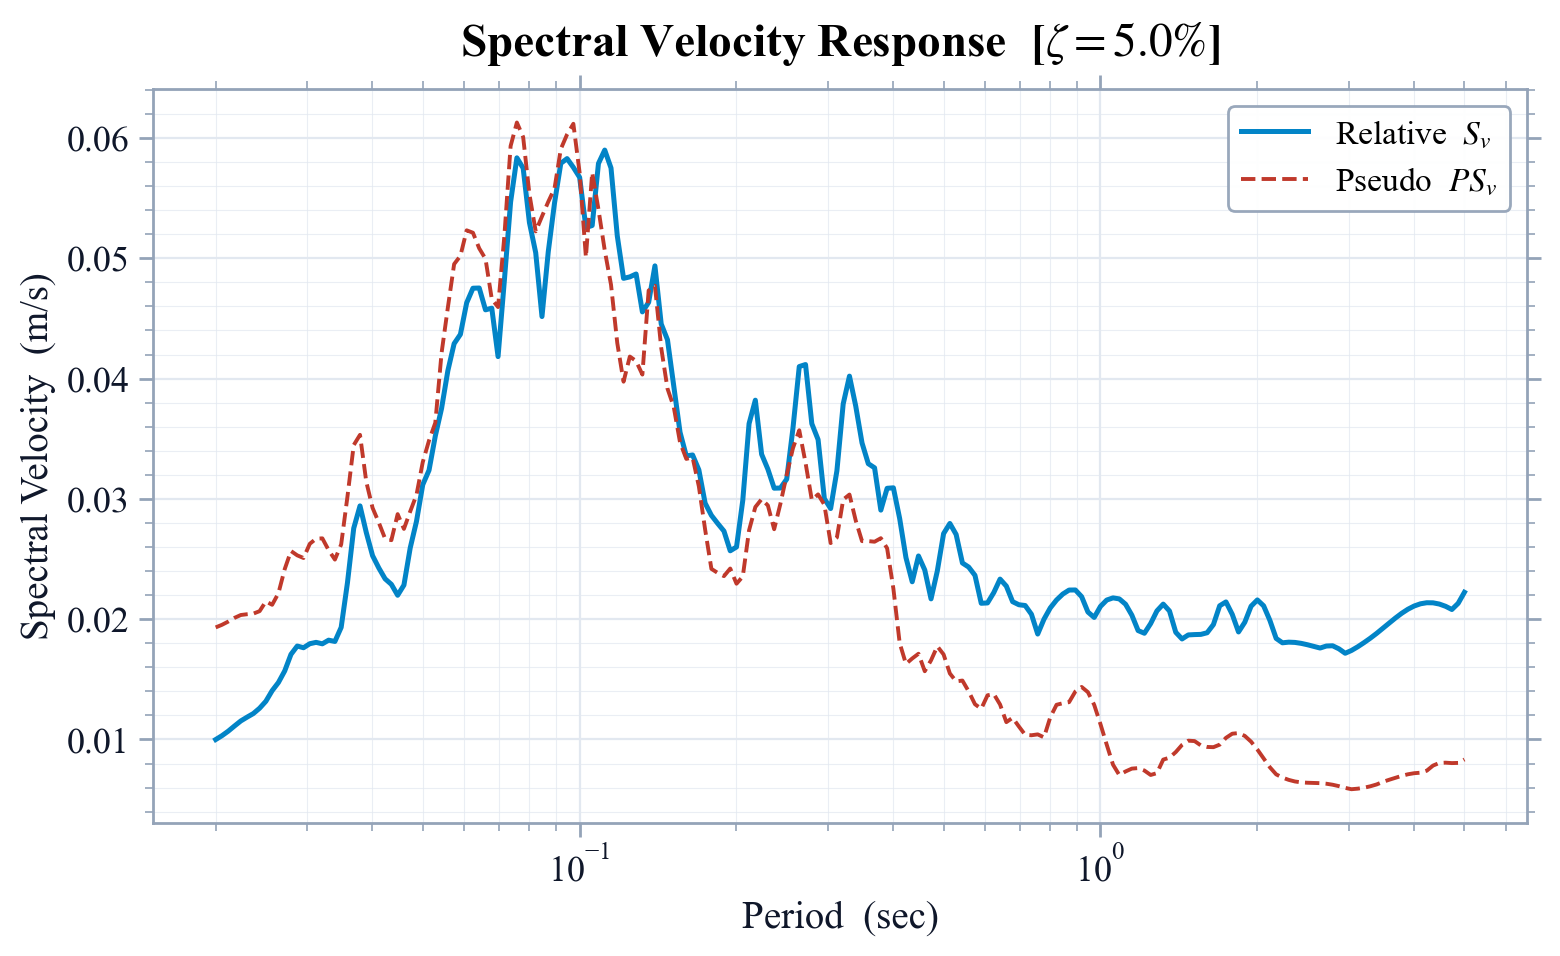
\includegraphics[width=0.85\linewidth]{spectral_velocity.png}
\caption{Spectral velocity at $\zeta=5\%$: relative $S_v$ (solid) and
pseudo $PS_v$ (dashed).}
\label{fig:sv}
\end{figure}

\paragraph{Observations.}
\begin{itemize}[leftmargin=1.4em,itemsep=0.15em]
  \item Both curves rise sharply from zero, reach a broad peak in the
        high-frequency range and then decay.
  \item Peak relative velocity:
        $S_{v,\max} \approx \SI{59.0}{mm/s}$ at $T \approx \SI{0.11}{s}$.
  \item Peak pseudo velocity:
        $PS_{v,\max} \approx \SI{61.3}{mm/s}$ at $T \approx \SI{0.08}{s}$.
  \item The two curves agree to within a few percent in the short-period
        range, confirming the consistency of the numerical solution; at
        long periods $PS_v$ decreases faster than $S_v$, which is the
        expected behaviour for lightly damped systems.
\end{itemize}

% =============================================================================
\section{Spectral acceleration, $S_a(T)$ and $PS_a(T)$}
\label{sec:sa}

The spectral acceleration is the primary input for force-based design
methods: the design lateral force on a single-mode-dominated structure
is taken proportional to $S_a(T_1)$, the spectral acceleration at the
fundamental period $T_1$. Figure~\ref{fig:sa} compares the absolute
spectrum $S_a(T)$ with its pseudo counterpart $PS_a(T)$.

\begin{figure}[h]
\centering
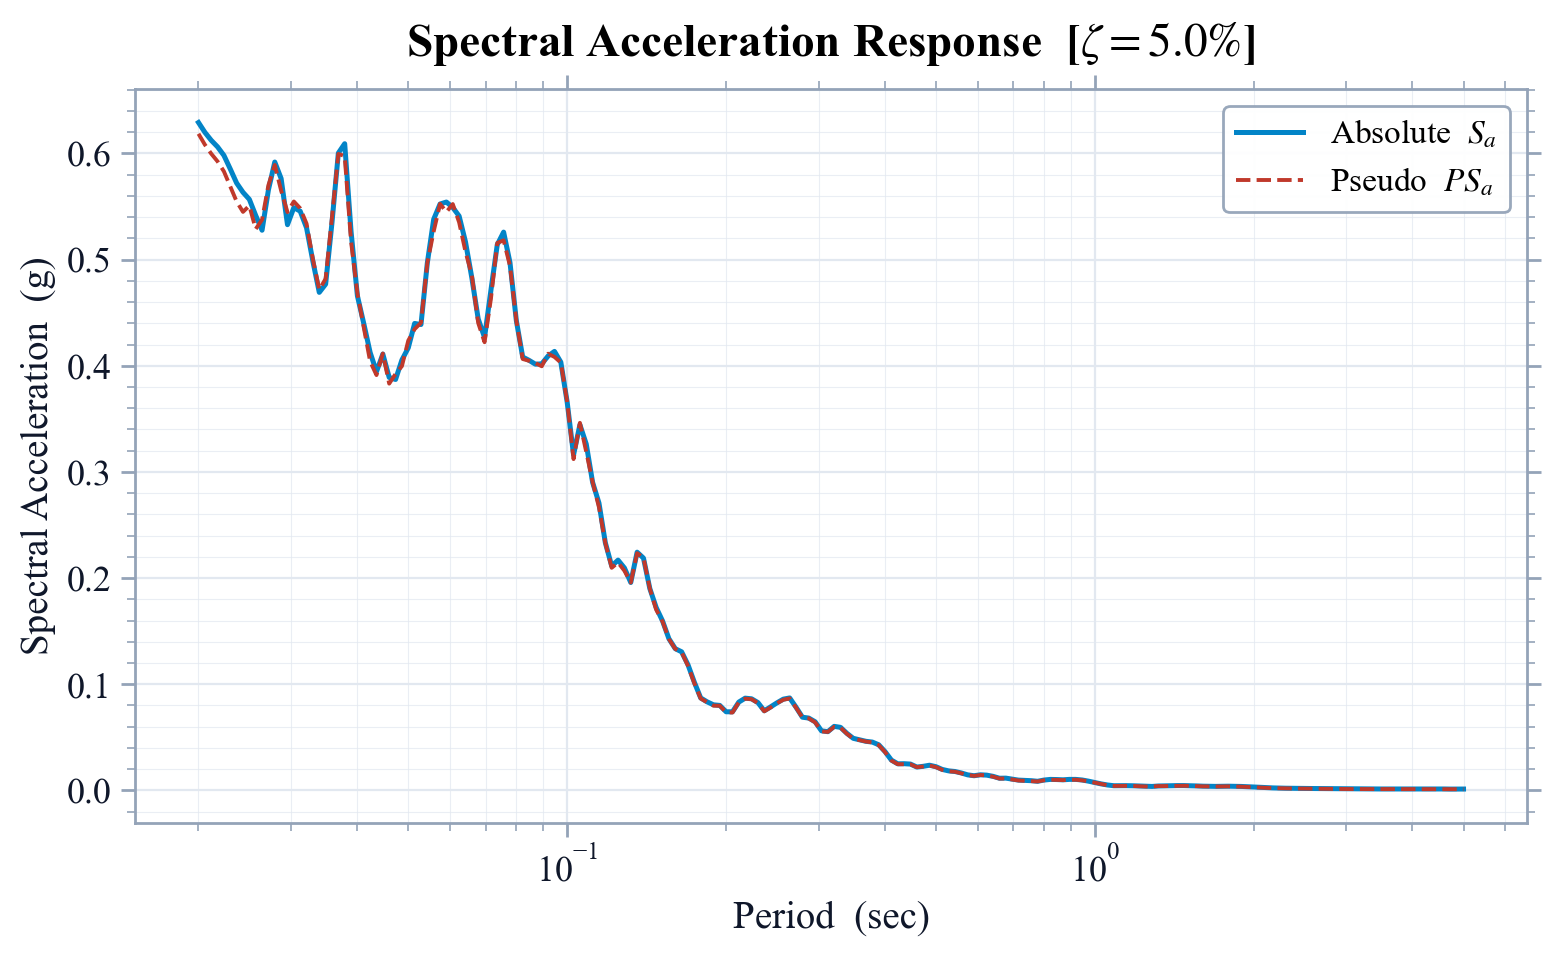
\includegraphics[width=0.85\linewidth]{spectral_acceleration.png}
\caption{Spectral acceleration at $\zeta=5\%$: absolute $S_a$ (solid)
and pseudo $PS_a$ (dashed).}
\label{fig:sa}
\end{figure}

\paragraph{Legend convention.}
Throughout this report the colour and line-style scheme is consistent:
\begin{center}\small
\begin{tabular}{@{}lll@{}}
\toprule
\textbf{Quantity} & \textbf{Line} & \textbf{Notation} \\
\midrule
Absolute spectral acceleration & solid sky-blue                & $S_a$  \\
Pseudo spectral acceleration   & dashed red                    & $PS_a$ \\
\bottomrule
\end{tabular}
\end{center}

\paragraph{Observations.}
\begin{itemize}[leftmargin=1.4em,itemsep=0.15em]
  \item Both spectra approach the PGA in the very short-period range,
        consistent with the well-known boundary condition
        $S_a(T \to 0) \to \mathrm{PGA}$.
  \item Peak values:
        $S_{a,\max} \approx \SI{0.629}{g}$ and
        $PS_{a,\max} \approx \SI{0.619}{g}$, both occurring at
        $T \approx \SI{0.02}{s}$.
  \item The two curves are visually indistinguishable up to
        $T \approx \SI{1}{s}$, with relative differences below
        $\sim 2\%$. This is the expected behaviour at $\zeta=5\%$ and
        validates the routine use of $PS_a$ in code spectra.
  \item Selected ordinates of engineering interest are listed in
        Table~\ref{tab:sa-vals}.
\end{itemize}

\begin{table}[h]
\centering
\caption{Selected spectral acceleration ordinates ($\zeta=5\%$).}
\label{tab:sa-vals}
\begin{tabular}{S[table-format=1.2]S[table-format=1.3]S[table-format=1.3]}
\toprule
{$T$ (s)} & {$S_a$ ($g$)} & {$PS_a$ ($g$)} \\
\midrule
0.02 & 0.629 & 0.619 \\
0.20 & 0.074 & 0.073 \\
0.30 & 0.056 & 0.055 \\
1.00 & 0.0073 & 0.0072 \\
2.00 & 0.0032 & 0.0032 \\
\bottomrule
\end{tabular}
\end{table}

% =============================================================================
\section{Discussion}
\label{sec:disc}

\subsection{Frequency content}
The combination of a comparatively high PGA (\SI{0.71}{g}) with very
small spectral displacements ($S_d < \SI{7}{mm}$ even at $T=\SI{5}{s}$)
indicates a record dominated by \emph{high-frequency content}. The
spectral acceleration drops by more than two orders of magnitude between
$T=\SI{0.02}{s}$ and $T=\SI{2}{s}$, with the bulk of the energy
concentrated below $T \approx \SI{0.2}{s}$ (i.e. above about \SI{5}{Hz}).
Such characteristics are typical of:
\begin{itemize}[leftmargin=1.4em,itemsep=0.15em]
  \item small-to-moderate near-field earthquakes recorded on rock,
  \item heavily filtered or windowed synthetic records, or
  \item engineering records used for the assessment of stiff structures
        such as nuclear safety-related equipment or low-rise rigid
        buildings.
\end{itemize}

\subsection{Implications for design}
\begin{itemize}[leftmargin=1.4em,itemsep=0.15em]
  \item \textbf{Stiff structures} ($T_1 \le \SI{0.3}{s}$): subjected
        to comparatively large base shears - $S_a$ between
        \SI{0.05}{g} and \SI{0.6}{g}, with the worst case in the
        rigid range.
  \item \textbf{Mid-rise structures} ($T_1 \approx \SI{0.5}{s}-\SI{1.5}{s}$):
        receive modest spectral demands, $S_a \le \SI{0.03}{g}$, and
        very small displacement demands.
  \item \textbf{Flexible/tall structures} ($T_1 > \SI{2}{s}$): excited
        only marginally by this record.
\end{itemize}

\subsection{Quality checks performed}
\begin{enumerate}[leftmargin=1.4em,itemsep=0.15em]
  \item $S_a$ and $PS_a$ agree to better than $\sim 2\%$ for
        $T \ge \SI{0.1}{s}$, which is the theoretical bound for
        $\zeta = 5\%$.
  \item $S_a(T \to 0)$ approaches the PGA, satisfying the rigid-body
        limit.
  \item $PS_v \to 0$ as $T \to 0$ and $PS_a \to 0$ as $T \to \infty$,
        in line with the limit behaviour of the pseudo-spectra.
\end{enumerate}

% =============================================================================
\section{Conclusions}

\begin{enumerate}[leftmargin=1.4em,itemsep=0.15em]
  \item A complete linear-elastic seismic response analysis at
        $\zeta=5\%$ has been carried out on the supplied record using
        the Nigam--Jennings exact piecewise-linear algorithm.
  \item The record exhibits a PGA of \SI{0.713}{g} and is strongly
        dominated by high-frequency content; spectral demands decrease
        rapidly with period.
  \item Maximum spectral ordinates:
        $S_{a,\max} \approx \SI{0.629}{g}$ at $T = \SI{0.02}{s}$,
        $S_{v,\max} \approx \SI{59}{mm/s}$ at $T \approx \SI{0.11}{s}$,
        $S_{d,\max} \approx \SI{6.6}{mm}$ at $T = \SI{5.0}{s}$.
  \item Pseudo and absolute spectra coincide to within a few percent in
        the engineering range $T \in [0.1,\,2.0]\,\mathrm{s}$,
        confirming the consistency of the numerical scheme and the
        validity of using $PS_a$ as a design ordinate.
  \item The tabulated spectra produced by the analysis can be used
        directly in modal-response-spectrum analyses of
        multi-degree-of-freedom structures.
\end{enumerate}

% =============================================================================
\appendix
\section{Computational implementation}
\label{app:code}

This appendix presents the complete Python implementation used to
perform the analysis described in the body of the report. The script
is self-contained: given the raw ground acceleration record it
produces the time-history plot, the three response-spectrum plots
and a tabulated output of every spectral ordinate.

\subsection{Program organisation}
The code is organised into five logically distinct blocks, summarised
below:

\begin{enumerate}[leftmargin=1.4em,itemsep=0.2em]
  \item \textbf{Configuration block.} Defines the global analysis
        parameters - sampling interval $\Delta t$, input units,
        gravitational acceleration $g$, damping ratio $\zeta$, and
        the number and range of natural periods. Concentrating these
        constants at the top makes the entire analysis trivially
        re-parametrisable.
  \item \textbf{Record ingestion.} Loads the single-column
        acceleration record, converts it from $g$ to SI units, and
        builds the corresponding time vector. The peak ground
        acceleration is reported on screen as a sanity check.
  \item \textbf{SDOF solver.} The function
        \texttt{sdof\_response\_spectra} implements the
        Nigam--Jennings exact piecewise-linear scheme. For each
        target period $T$:
        \begin{itemize}[leftmargin=1.4em,itemsep=0.1em]
          \item the natural and damped circular frequencies
                $\omega_n, \omega_d$ and the discrete transition
                coefficients are formed from closed-form expressions;
          \item the relative displacement history $u(t)$ is obtained
                by marching the $2\times 2$ state recurrence in time;
          \item the relative velocity $\dot{u}(t)$ is recovered by
                centred finite differences;
          \item the absolute (total) acceleration is reconstructed
                from the equation of motion as
                $\ddot{u}_t = -(2\zeta\omega_n\dot{u} + \omega_n^2 u)$,
                which enforces dynamic equilibrium exactly;
          \item the peak absolute values give $S_d$, $S_v$ and the
                absolute $S_a$ for that period.
        \end{itemize}
        The pseudo ordinates are then obtained algebraically from
        $S_d$ as $PS_v = \omega_n S_d$ and $PS_a = \omega_n^2 S_d$.
  \item \textbf{Tabulation.} The five spectral arrays and the period
        vector are stacked column-wise and written to a CSV file with
        a self-describing header, ready for use in spreadsheets or
        structural-analysis software.
  \item \textbf{Plotting block.} A bespoke Matplotlib style sheet
        emulating the look of the project's web dashboard is applied
        (serif typography, light grid, mirrored axis box, soft
        sky-blue primary trace, dashed red accent trace). Four
        figures are produced: the ground-acceleration time history
        and the three response spectra, with absolute / pseudo
        comparisons where applicable.
\end{enumerate}

\subsection{Key implementation choices}
\begin{itemize}[leftmargin=1.4em,itemsep=0.2em]
  \item \textbf{Logarithmic period grid.} 200 points spaced
        logarithmically between \SI{0.02}{s} and \SI{5}{s} provide
        dense resolution at short periods (where spectra vary
        rapidly) without wasting points in the long-period tail.
  \item \textbf{Exact piecewise-linear integration.} Unlike
        Newmark-$\beta$, the Nigam--Jennings recurrence has no
        period-dependent dispersion error, which is essential when
        $\Delta t / T$ becomes large for short-period oscillators.
  \item \textbf{Equation-of-motion reconstruction of $\ddot{u}_t$.}
        Computing the absolute acceleration directly from the
        relative displacement and velocity via the equation of motion
        guarantees that the residual
        $\ddot{u}_t + 2\zeta\omega_n\dot{u} + \omega_n^{\,2} u = 0$
        vanishes identically, eliminating one common source of error
        in response-spectrum routines.
  \item \textbf{Single source of styling.} All figure aesthetics are
        controlled through a single \texttt{rcParams} block and a
        helper function applied to every axis, ensuring a uniform
        appearance across all plots.
\end{itemize}

\subsection{Complete source listing}
The full script is reproduced verbatim below.

\lstinputlisting[language=Python]{generate_spectra.py}

\vspace{1em}
{\color{rule}\rule{\linewidth}{0.4pt}}\\
{\small \emph{End of report.}}

\end{document}
